\marklabel{sec:opt-cpanel}
{
\section {OPT\_CPANEL}
}

\subsection{Introduction}

Ce paquetage permet la connexion de quatre boutons poussoir sur le port série
du routeur fli4l. En appuyant sur l'un des boutons vous déclenchez une commande
système par exemple arrêter ou redémarrer. Les boutons peuvent être affectés
librement. 14 variantes sont possibles (en théorie 15 variantes mais avec la
15ème le système ne répond pas)

La LED2 power s'allume en vert lorsque le circuit est prêt à l'emploi.
Lorsqu'une commande est exécutée, la LED clignotera. La LED1 peut être
assignée librement, (pour plus d'informations voir ci-dessous).

\subsection{Les boutons poussoir}

Voici les affectations des boutons correspondent aux valeur.

\begin{itemize}
    \item bouton 1 = 1
    \item bouton 2 = 2
    \item bouton 3 = 4
    \item bouton 4 = 8
\end{itemize}

Si plusieurs boutons sont pressées simultanément, les valeurs des boutons seront
ajoutées. Le nombre obtenu sera utilisé pour affecter une commande.

Les commandes à exécuter sont à paramétrer dans cette variable~:
\var{OPT\_CPANEL\_FUNKTION1}='COMMANDE'
Il convient de noter que pour certaines commandes, vous devez spécifier le
chemin complet vers le programme ou le script.

Voici quelques exemples~:
\begin{verbatim}

fli4lctrl dial pppoe    Connexion du modem DSL
fli4lctrl hangup pppoe  Déconnexion du modem DSL
isdnctrl dial ippp0     Connexion du modem ISDN
isdnctrl hangup ippp0   Déconnexion du modem ISDN
/sbin/reboot            Redémarrer le routeur
/sbin/halt              Arrêter le routeur

\end{verbatim}

\subsection{Affichage de l'état de la configuration}

Il y a quatre façons d'indiquer l'état de la LED.

DSL~: 

Affiche uniquement l'état de la connexion DSL.

ISDN~: 

Affiche l'état de la connexion ISDN. Si au moins un canal ISDN est en ligne,
la première LED1 sera allumée.

DSLISDN~:

Affiche l'état de la connexion DSL et ISDN avec en plus un ou tous les canaux
en lignes.

SCRIPT~:
% Synchronized to r30045
Ici, vous pouvez créer votre propre requête. Faite attention à se qui suit~:
\begin{itemize}
    \item Vous devez saisir que des commandes.
    \item \#!/bin/sh doit être automatiquement inséré au début du script.
    \item Pour allumer la première LED1, vous devez indiquer 'on' dans le fichier
          /var/run/cpanel.status, (bien sûr sans les ' ').
    \item Pour éteindre la LED, vous devez indiquer 'off' dans le fichier
          /var/run/cpanel.status.
    \item Pour faire 'clignoter', vous ne devez rien indiquer dans le
          fichier /var/run/cpanel.status, la LED1 clignote jusqu'au réglage
          suivant 'off' ou 'on'
\end{itemize}

Exemple~:

Cette configuration interroge l'état du DSL~:
\begin{verbatim}
echo off > /var/run/cpanel.status
fli4lctrl status | grep online >/dev/null && echo on > /var/run/cpanel.status
\end{verbatim}
Attention~: 
Vous devez Insérer les paramètres seulement si vous savez ce que vous faites.
Une configuration défectueux peut causer un mauvais fonctionnement du cPanel, il
peut ne pas démarrer.

\subsection{Dépannage}
\subsubsection{Hardware}

Si ca ne fonctionne pas du premier coup, vérifiez d'abord votre circuit. Faites
attention aux brochage correct sur le connecteur du PC. Si votre routeur dispose
encore d'un port série à 25 broches, le brochage est différent de celui du
dessin de circuit~! Si vous n'avez pas trouvé d'erreur dans votre circuit,
vérifiez le câble de la prise serie à la carte mère. Étant donné que les
fabricants de cartes mères ne sont pas tous d'accord sur une norme. Si
nécessaire, vérifier l'affectation des broches du connecteur série avec le
brochage du connecteur de la carte mère (voir le manuel de votre carte mère).

\subsubsection{Software}

Vérifiez d'abord, si le logiciel cPanel est bien démarré lors du démarrage du
routeur. Cela peut se vérifier, vers la fin de l'installation un message sera
affiché. Si ce n'est pas le cas ou si vous avez manqué le message, l'état peut
être contrôlé avec les touches "ps ax' sur la console. Si cPanel n'est pas dans
la liste, vous avez probablement oublié d'activer dans le fichier config/cpanel.txt
la variable \var{OPT\_CPANEL}='yes' elle est resté sur 'no'.\\
Une autre source d'erreur pourrait être la carte graphique. Si vous avez une
carte graphique dans votre routeur, le premier port série (COM1) est peut être
utilisé pour la console. Vous devez modifier la variable \var{CPANEL\_PORT}='/dev/ttyS0'
par '/dev/ttyS1' dans le fichier config/cpanel.txt, bien entendu, le circuit doit
être connecté au COM2.

\subsection{Généralité}

  \begin{figure}[htbp]
    \centering
    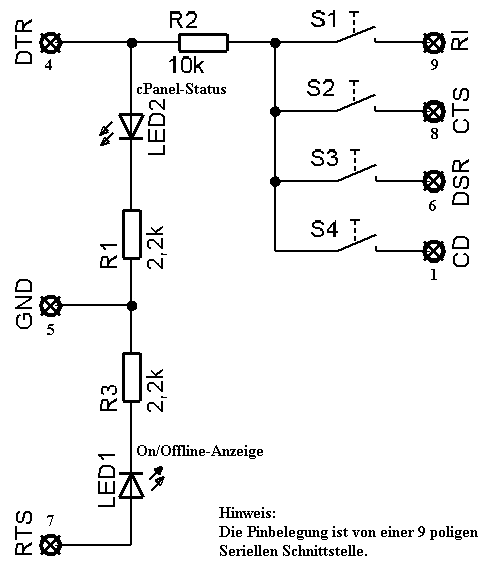
\includegraphics[width=485pt]{schematic}
    \caption{Schéma du circuit de commande}
    \label{fig:schaltplan}
  \end{figure}


\wichtig{Je décline toute responsabilité pour tout dommage causé!}

S'il vous plaît vous pouvez poster dans le newsgroup slpine.fli4l.opt vos
problèmes, vos suggestions et vos réussites.

Merci d'avoir lu cette documentation. Maintenant, je ne peux que vous
souhaitez beaucoup de plaisir à utiliser cPanel.
